% Options for packages loaded elsewhere
\PassOptionsToPackage{unicode}{hyperref}
\PassOptionsToPackage{hyphens}{url}
%
\documentclass[
]{book}
\usepackage{amsmath,amssymb}
\usepackage{lmodern}
\usepackage{ifxetex,ifluatex}
\ifnum 0\ifxetex 1\fi\ifluatex 1\fi=0 % if pdftex
  \usepackage[T1]{fontenc}
  \usepackage[utf8]{inputenc}
  \usepackage{textcomp} % provide euro and other symbols
\else % if luatex or xetex
  \usepackage{unicode-math}
  \defaultfontfeatures{Scale=MatchLowercase}
  \defaultfontfeatures[\rmfamily]{Ligatures=TeX,Scale=1}
\fi
% Use upquote if available, for straight quotes in verbatim environments
\IfFileExists{upquote.sty}{\usepackage{upquote}}{}
\IfFileExists{microtype.sty}{% use microtype if available
  \usepackage[]{microtype}
  \UseMicrotypeSet[protrusion]{basicmath} % disable protrusion for tt fonts
}{}
\makeatletter
\@ifundefined{KOMAClassName}{% if non-KOMA class
  \IfFileExists{parskip.sty}{%
    \usepackage{parskip}
  }{% else
    \setlength{\parindent}{0pt}
    \setlength{\parskip}{6pt plus 2pt minus 1pt}}
}{% if KOMA class
  \KOMAoptions{parskip=half}}
\makeatother
\usepackage{xcolor}
\IfFileExists{xurl.sty}{\usepackage{xurl}}{} % add URL line breaks if available
\IfFileExists{bookmark.sty}{\usepackage{bookmark}}{\usepackage{hyperref}}
\hypersetup{
  pdftitle={Modelos Matemáticos en Ecología I},
  pdfauthor={Gerardo Martín},
  hidelinks,
  pdfcreator={LaTeX via pandoc}}
\urlstyle{same} % disable monospaced font for URLs
\usepackage{longtable,booktabs,array}
\usepackage{calc} % for calculating minipage widths
% Correct order of tables after \paragraph or \subparagraph
\usepackage{etoolbox}
\makeatletter
\patchcmd\longtable{\par}{\if@noskipsec\mbox{}\fi\par}{}{}
\makeatother
% Allow footnotes in longtable head/foot
\IfFileExists{footnotehyper.sty}{\usepackage{footnotehyper}}{\usepackage{footnote}}
\makesavenoteenv{longtable}
\usepackage{graphicx}
\makeatletter
\def\maxwidth{\ifdim\Gin@nat@width>\linewidth\linewidth\else\Gin@nat@width\fi}
\def\maxheight{\ifdim\Gin@nat@height>\textheight\textheight\else\Gin@nat@height\fi}
\makeatother
% Scale images if necessary, so that they will not overflow the page
% margins by default, and it is still possible to overwrite the defaults
% using explicit options in \includegraphics[width, height, ...]{}
\setkeys{Gin}{width=\maxwidth,height=\maxheight,keepaspectratio}
% Set default figure placement to htbp
\makeatletter
\def\fps@figure{htbp}
\makeatother
\setlength{\emergencystretch}{3em} % prevent overfull lines
\providecommand{\tightlist}{%
  \setlength{\itemsep}{0pt}\setlength{\parskip}{0pt}}
\setcounter{secnumdepth}{5}
\usepackage{booktabs}
\ifluatex
  \usepackage{selnolig}  % disable illegal ligatures
\fi
\usepackage[]{natbib}
\bibliographystyle{apalike}

\title{Modelos Matemáticos en Ecología I}
\author{Gerardo Martín}
\date{2021-07-29}

\begin{document}
\maketitle

{
\setcounter{tocdepth}{1}
\tableofcontents
}
\hypertarget{sobre-este-curso}{%
\chapter{Sobre este curso}\label{sobre-este-curso}}

En el curso \textbf{Modelos matemáticos en ecología} aprenderemos a utilizar algunas herramientas matemáticas para entender procesos en ecología. Los contenidos del índice se apegan al \href{Programa-curso.pdf}{programa completo del curso}, el cual se impartirá en los \href{Horario.pdf}{horarios normales establecidos}. Para conocer cuándo, cómo y qué temas se se impartirán puedes consultar la \href{Estrategia-docente.pdf}{estrategia docente}.

\hypertarget{criterios-de-evaluaciuxf3n}{%
\chapter{Criterios de evaluación}\label{criterios-de-evaluaciuxf3n}}

Las constribuciones a cada calificación parcial serán por igual (25\% cada uno):

\begin{itemize}
\tightlist
\item
  Asistencia
\item
  Trabajos de clase cumplidos
\item
  Participación
\item
  Examen
\end{itemize}

\hypertarget{unidad-i-introducciuxf3n-a-la-modelaciuxf3n}{%
\chapter{Unidad I: Introducción a la modelación}\label{unidad-i-introducciuxf3n-a-la-modelaciuxf3n}}

\hypertarget{introducciuxf3n-al-concepto-de-modelo-matemuxe1tico}{%
\section{Introducción al concepto de modelo matemático}\label{introducciuxf3n-al-concepto-de-modelo-matemuxe1tico}}

Imaginemos a seis personas invidentes, con la tarea de encontrar qué es el objeto que está frente a ellas usando únicamente el tacto. En la parábola de los seis hombres ciegos, el objeto es un elefante, de modo que la imágen que cada uno de ellos se forma del objeto depende enteramente de la parte del elefante que están tocando.

\begin{figure}

{\centering 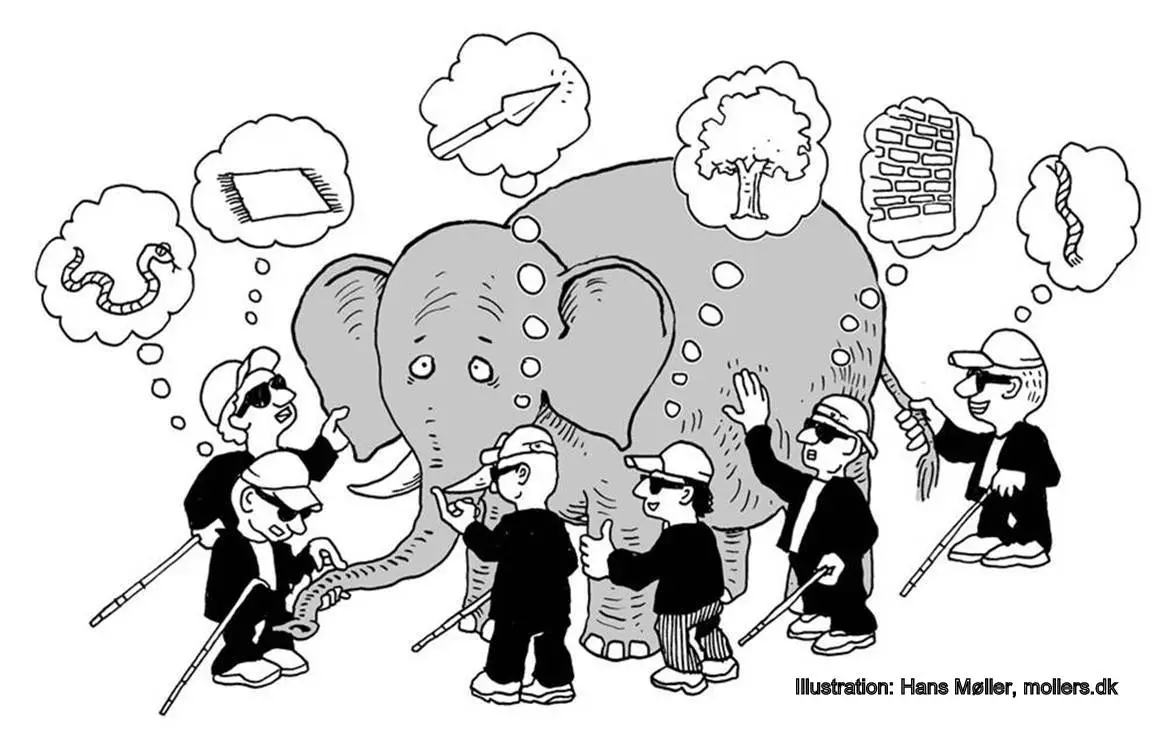
\includegraphics[width=16.17in]{Unidad-I/elefante} 

}

\caption{La parábola de los seis hombres ciegos inspeccionando un elefante.}\label{fig:unnamed-chunk-5}
\end{figure}

Quien toque los colmillos podrá pensar que se trata de una lanza, la trompa podría tratarse de una serpiente, la cola de una cuerda, las patas troncos de árbol y el cuerpo una pared. Es evidente que todas las hipótesis presentadas después de la inspección fueron erróneas, y que cuando estudiamos al mundo lo haremos igual, con la descripción de tan sólo una fracción de éste. Un séptimo hombre que pregunte a los otros seis qué fue lo que vieron podría formarse una imágen más completa del \emph{sistema} para proponer otra hipótesis: se trata de un objeto grande reposando sobre cuatro columnas con apéndices adelante y atrás.

Al estudiar los sistemas ecológicos, al igual que los ciegos, no sabremos que estamos frente a un elefante. Los sistemas ecológicos, al igual que los elefantes, también tienen componentes interconectados, y nosotros los ecólogos somos como los hombres ciegos, sólo podemos observar ciertas partes de los ecosistemas. En nuestro trabajo entonces, aprender a identificar y proponer hipótesis sobre cómo funcionan los sistemas ecológicos.

Las hipótesis propuestas por los seis hombres representan modelos, es decir simplificaciones del mundo que nos ayudan a entenderlo. Los modelos matemáticos son simplificaciones formales del mundo utilizando otro lenguaje, las matemáticas.

\hypertarget{cuxf3mo-construir-un-modelo}{%
\section{Cómo construir un modelo}\label{cuxf3mo-construir-un-modelo}}

¿Cómo se construye un modelo? Es una pregunta difícil de responder, pues difícilmente existe un sólo modo de hacerlo que funcione para \href{mailto:tod@s}{\nolinkurl{tod@s}}. Aquí voy a hablar de mi propia experiencia, y cómo aprendí a utilizar las matemáticas y estadística para entender los sistemas ecológicos. Los pasos generales que sigo son:

\begin{enumerate}
\def\labelenumi{\arabic{enumi}.}
\tightlist
\item
  Identificar el sistema y sus componentes
\item
  Crear un modelo conceptual, haciendo dibujos
\item
  Identificar las herramientas matemáticas disponibles para representar el modelo conceptual
\item
  Establecer objetivos claros y alcanzables
\item
  Proponer una serie de modelos alternativos
\item
  Determinar una estrategia para seleccionar uno solo de los modelos que propuse para logar el objetivo
\end{enumerate}

La estrategia general que les doy puede, por el momento, sonar un tanto abstracta, pero la iremos poniendo en práctica conforme avanza el curso para que al final, esperemos, tenga más sentido que ahorita.

\hypertarget{discusiuxf3n-sobre-las-distintas-herramientas-matemuxe1ticas-empleadas-en-la-modelaciuxf3n-matemuxe1tica}{%
\section{Discusión sobre las distintas herramientas matemáticas empleadas en la modelación matemática}\label{discusiuxf3n-sobre-las-distintas-herramientas-matemuxe1ticas-empleadas-en-la-modelaciuxf3n-matemuxe1tica}}

Las matemáticas son un área de conocimiento muy extenso, por lo que hablar de todas las herramientas disponibles ¡nos podría llevar años! En este curso nos vamos a enfocar en un tipo general de modelo y de sistema ecológico: aquellos que cambian rápidamente con el tiempo, también llamados dinámicos.

Las herramientas matemáticas más comunmente utilizadas para estudiar estos sistemas son las ecuaciones diferenciales ordinarias y el álgebra de matrices. Las ecuaciones diferenciales nos ayudan a medir los cambios que sufre el sistema ecológico a través del tiempo en cada uno de sus componentes, y son muy útiles para representar las ideas plasmadas en forma de modelos conceptuales. El álgebra de matrices, por otro lado, nos sirve para \emph{conectar} los cambios de los diferentes componentes del sistema de estudio, y así hacer cálculos sobre sus cambios \emph{como un todo}.

Como podemos ver, gran parte de este curso estará enfocado en \emph{entender y medir los cambios}. Te preguntarás entonces ¿cambios de qué? En ecología, estos son algunos de los cambios que nos interesa observar:

\begin{enumerate}
\def\labelenumi{\arabic{enumi}.}
\tightlist
\item
  Número de individuos de una especie
\item
  Cantidad de materia orgánica almacenada en la vegetación
\item
  Calorías consumidas por una población de aves
\item
  Probabilidad de extinción de una especie
\end{enumerate}

\hypertarget{uso-de-los-modelos-matemuxe1ticos-en-ecologuxeda}{%
\section{Uso de los modelos matemáticos en ecología}\label{uso-de-los-modelos-matemuxe1ticos-en-ecologuxeda}}

\hypertarget{tipos-de-modelos-en-ecologuxeda}{%
\section{Tipos de modelos en ecología}\label{tipos-de-modelos-en-ecologuxeda}}

\hypertarget{modelos-deterministas-generalidades}{%
\subsection{Modelos deterministas (generalidades)}\label{modelos-deterministas-generalidades}}

\hypertarget{modelos-estocuxe1sticos-generalidades}{%
\subsection{Modelos estocásticos (generalidades)}\label{modelos-estocuxe1sticos-generalidades}}

\hypertarget{methods}{%
\chapter{Methods}\label{methods}}

We describe our methods in this chapter.

\hypertarget{applications}{%
\chapter{Applications}\label{applications}}

Some \emph{significant} applications are demonstrated in this chapter.

\hypertarget{example-one}{%
\section{Example one}\label{example-one}}

\hypertarget{example-two}{%
\section{Example two}\label{example-two}}

  \bibliography{book.bib,packages.bib}

\end{document}
